\section*{Введение}
\addcontentsline{toc}{section}{Введение}
Данный документ призван познакомить читателей с результатами работы авторов над задачей создания системы управления для робота-машинки, которая бы давала ему способность автоматически (самостоятельно) выполнять параллельную парковку.

Более конкретно ее можно описать примерно так.

Имеется робот-машинка, ходовая часть которого устроена примерно так же, как у настоящего заднеприводного автомобиля: один из пары его двигателей приводит во вращение задние колеса, второй отвечает за поворот передних, рулевых колес.
Данный робот должен проехать вдоль возможного места парковки, обозначенного с помощью посторонних объектов, имитирующих собой другие стоящие неподвижно транспртные средства (см.~рисунок~\ref{img_test_zone_gen_view}), оценить его геометрические параметры, необходимые для совершения маневра, характерного для параллельной парковки, и, собственно, проделать последний.

\begin{figure}[h]
    \centering
    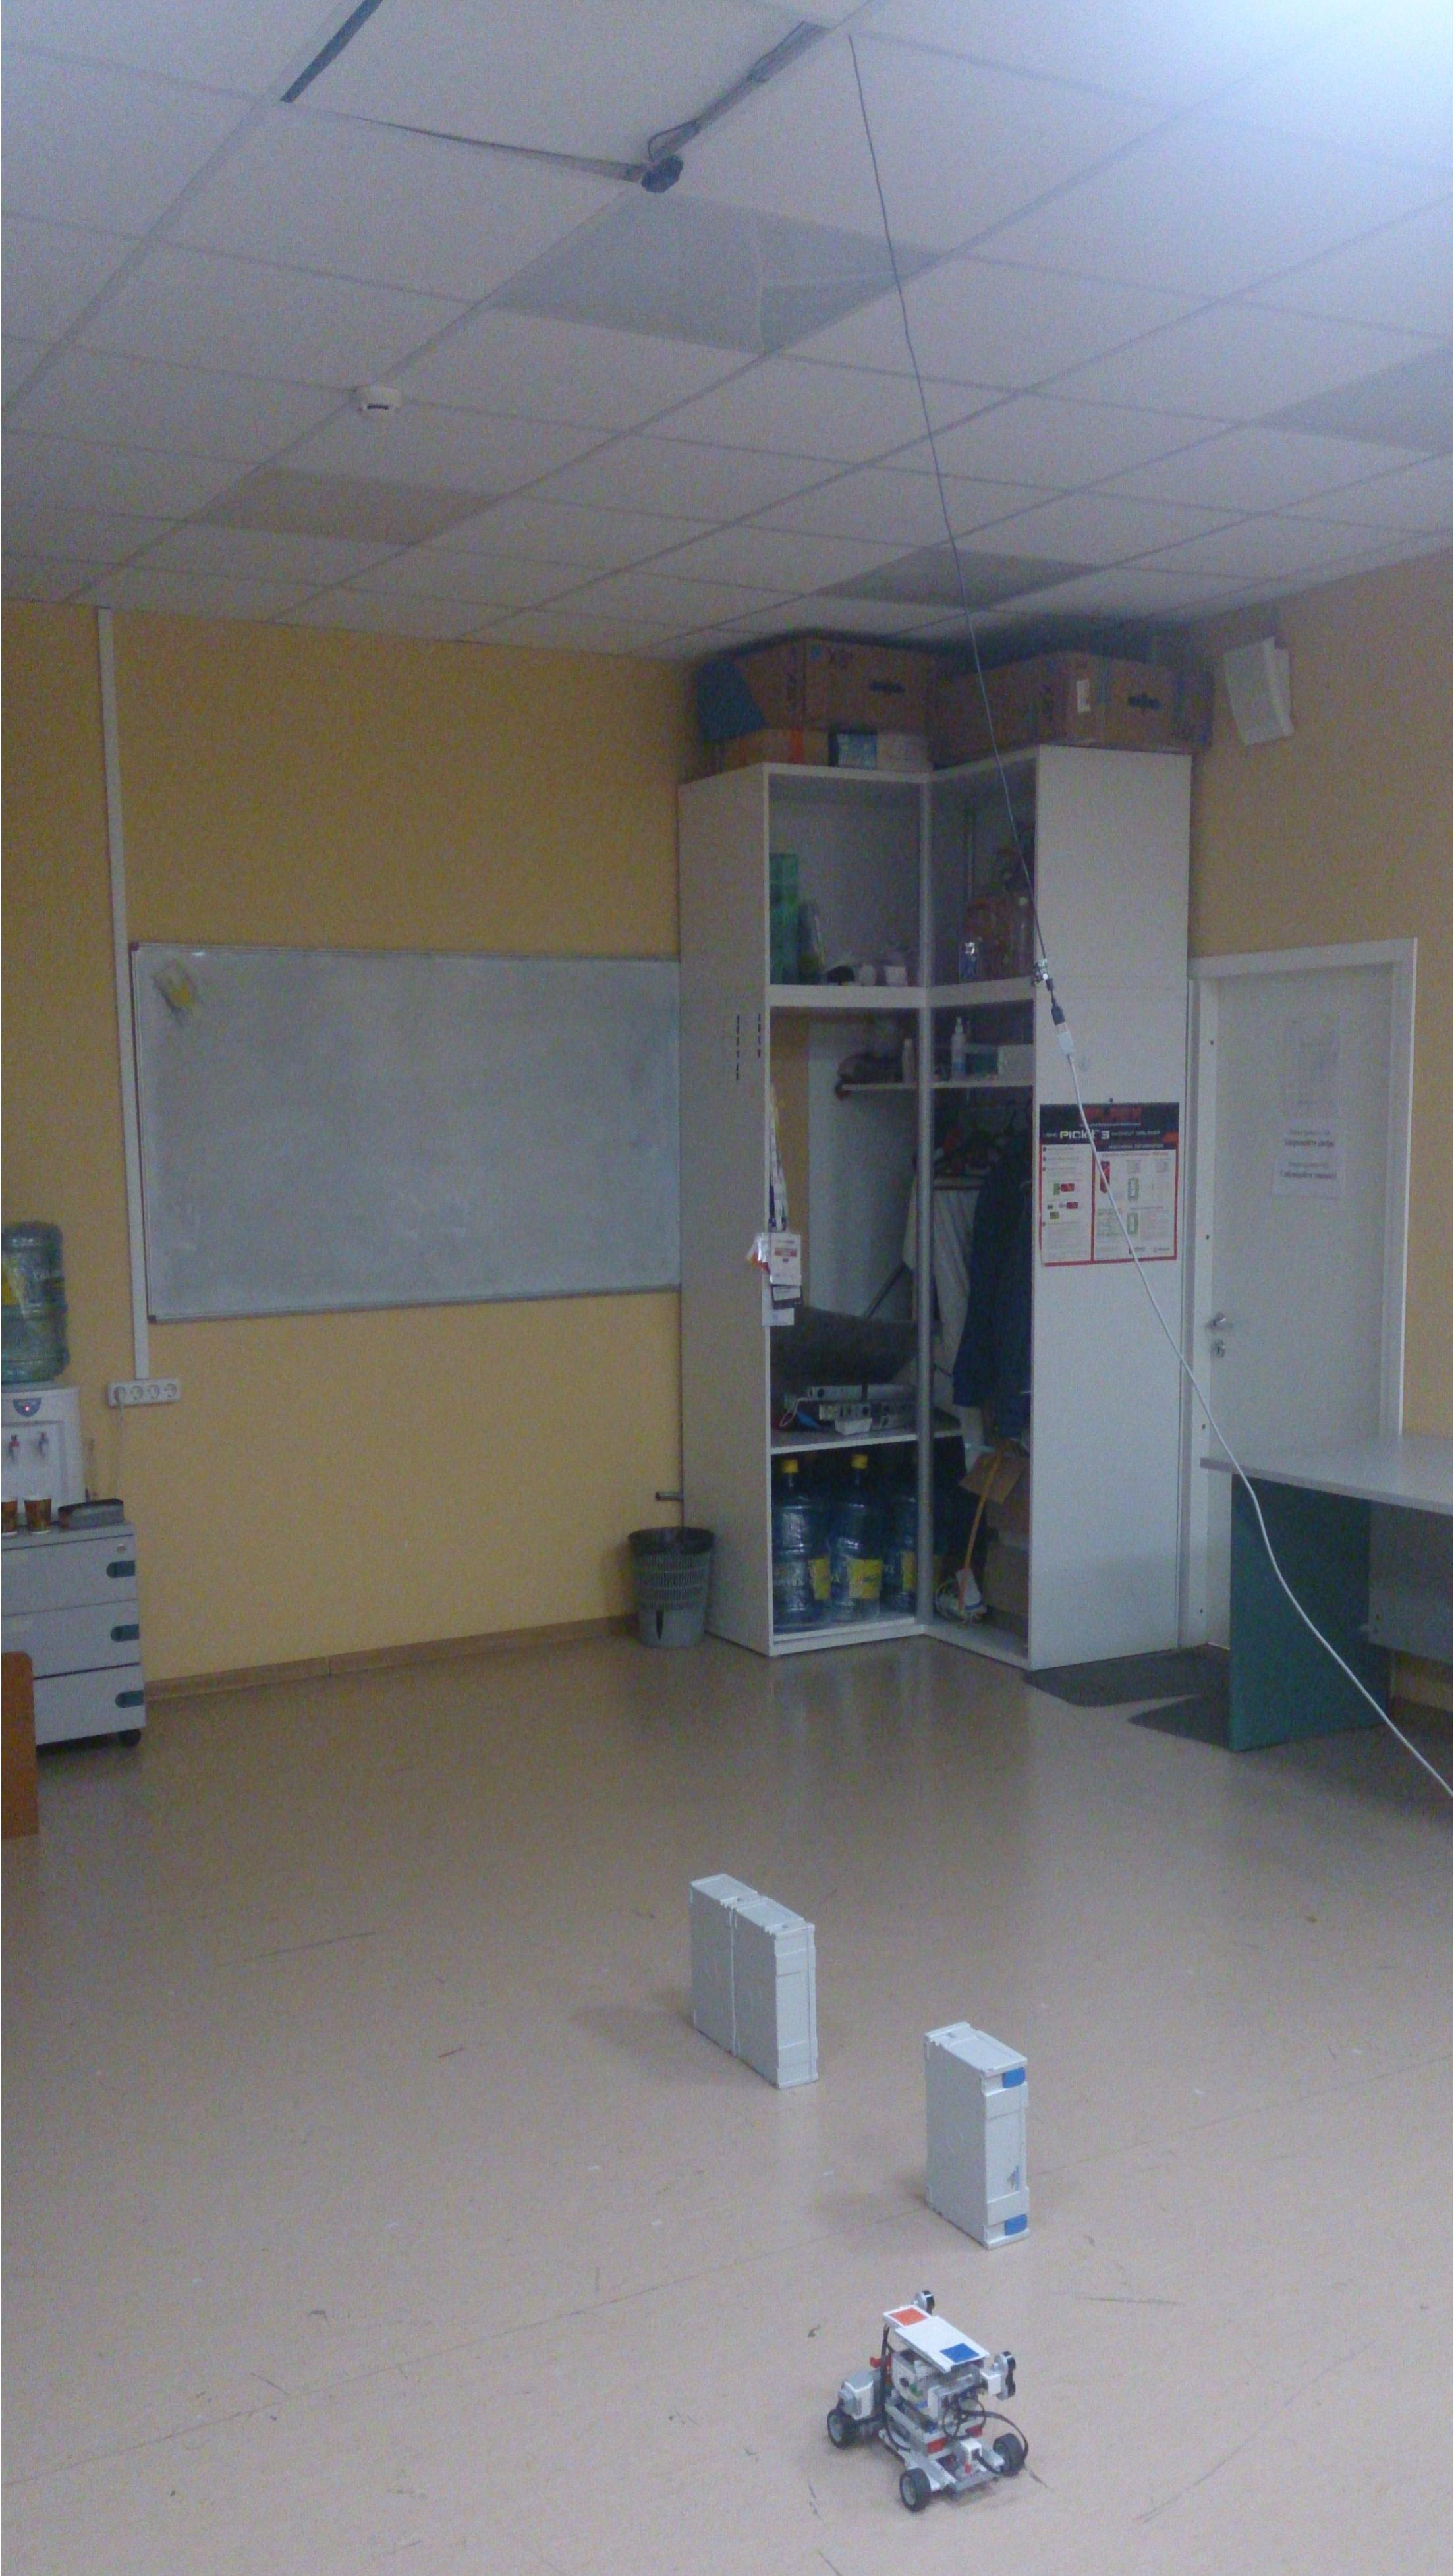
\includegraphics[width= 0.5\textwidth, draft]{test_zone_gen_view.jpg}
    \caption{Общий вид зоны проведения экспериментов.}
    \label{img_test_zone_gen_view}
\end{figure}

Для ее решения авторам пришлось проработать следующие технические вопросы:
\begin{itemize}
    \item создание упомянутого робота из конструктора LEGO Mindstorms EV3;
    \item подбор для него датчиков и программная реализация алгоритмов обработки поступающей с них информации;
    \item проектирование системы управления движением робота;
    \item создание алгоритма картирования парковочного места и его окрестностей.
\end{itemize}
Описанию их ключевых моментов и посвящена основная часть этого документа.


\newpage
\section{Особенности строения робота}
Зависимость между углом~$\varphi$ и $\varphi_1$ и $\varphi_2$~--- углами поворота левого и правого соответственно передних колес (незнакомые обозначения см. в следующем разделе):
\begin{equation}
    \tan\varphi = \cfrac{L \tan\varphi_1}{L - \cfrac{D}{2}\tan\varphi_1},
    \qquad
    \tan\varphi = \cfrac{L \tan\varphi_2}{L + \cfrac{D}{2}\tan\varphi_2},
\end{equation}
где $D$~--- расстояние на передней оси робота, показанное на рисунке~\ref{img_coll}.
\begin{figure}[h]
    \centering
    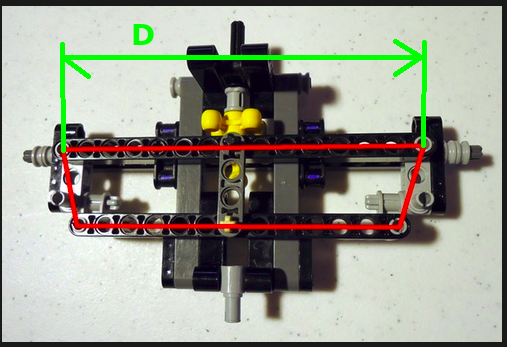
\includegraphics[width=\textwidth]{coll.png}
    \caption{Физический смысл длины $D$.}
    \label{img_coll}
\end{figure}



\newpage
\section{Управление движением робота}
\begin{figure}[h]
    \centering
    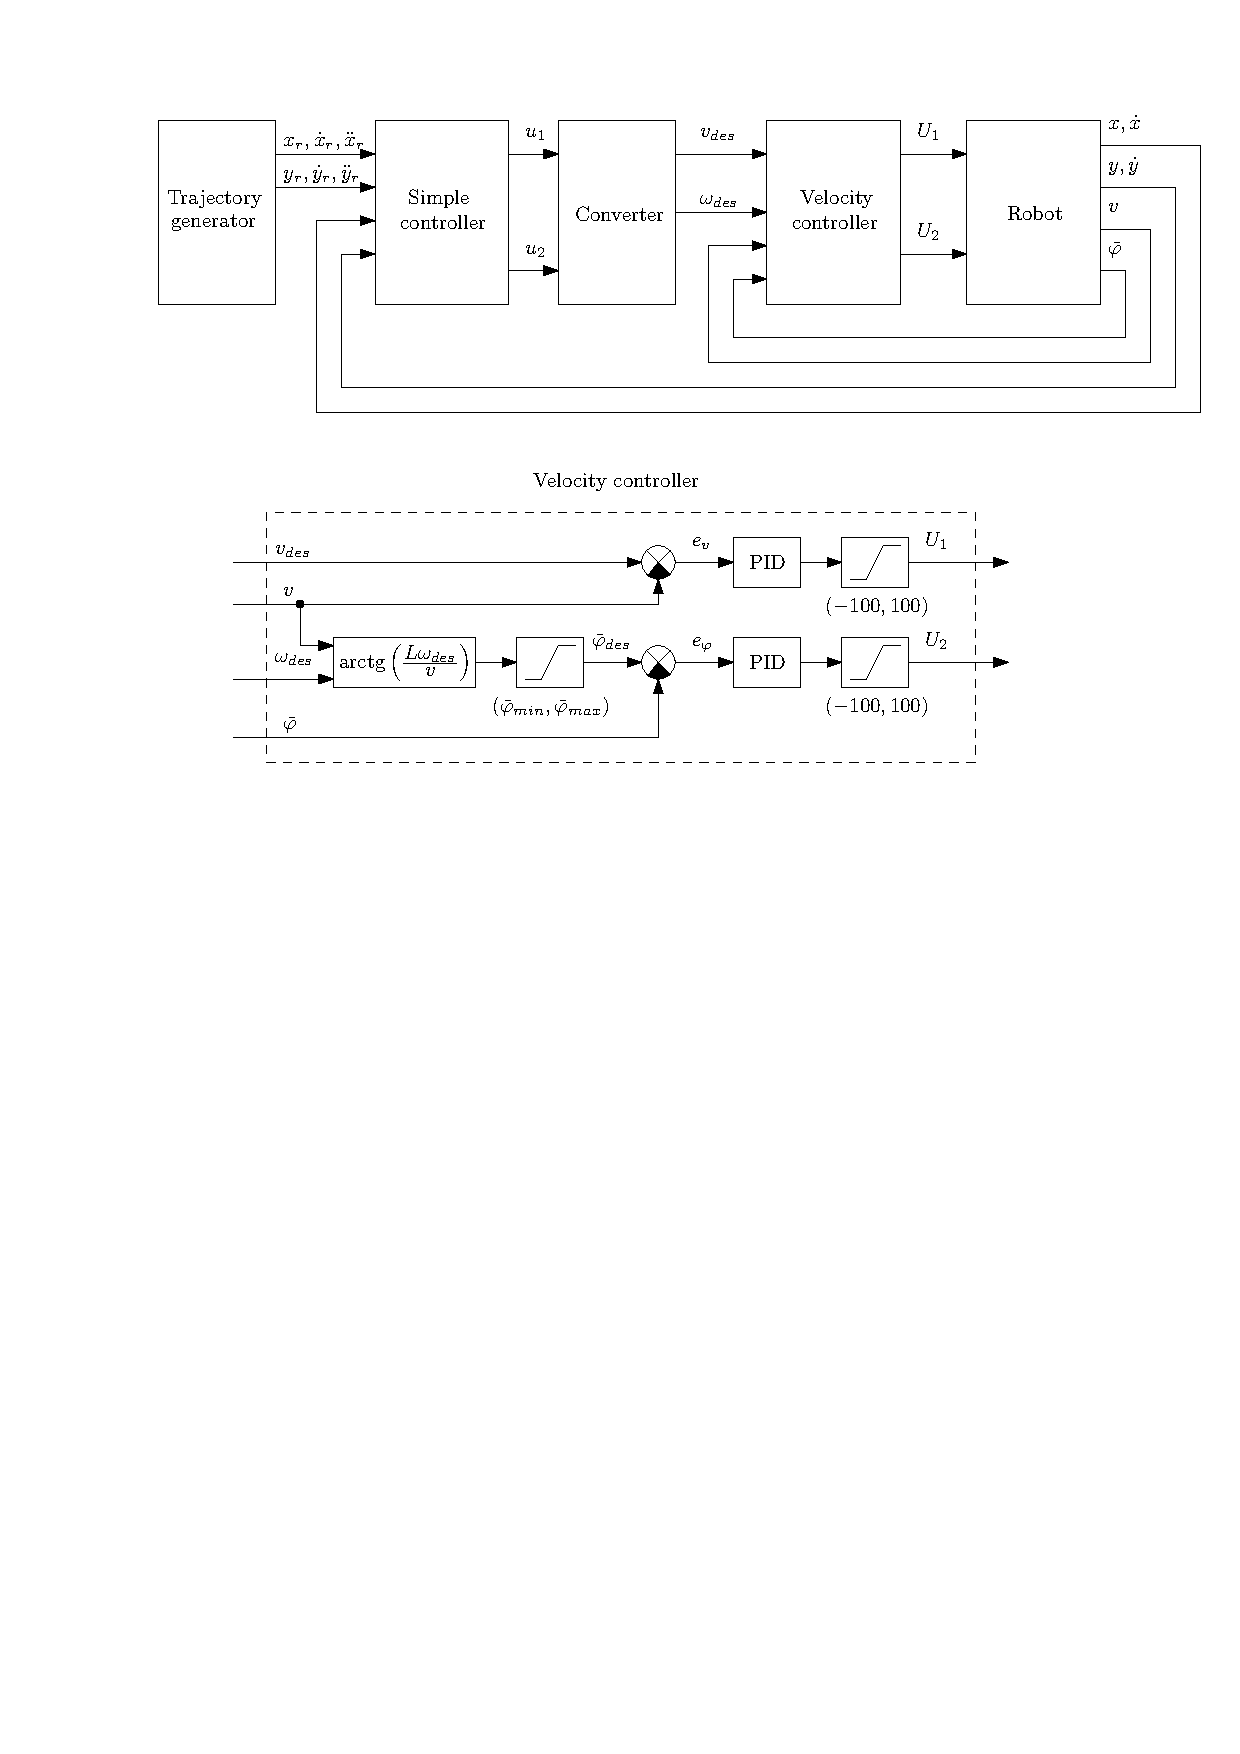
\includegraphics[width=\textwidth]{control_system.pdf}
    \caption{Структура системы управления движением робота.}
    \label{img_control_system}
\end{figure}
На рисунке~\ref{img_control_system}:\\
$U_1$~--- \% от максимального напряжения, подаваемого на двигатель, приводящий в движение задние колеса;\\
$U_2$~--- \% от максимального напряжения, подаваемого на рулевой двигатель;\\
$\bar\varphi$~--- угол поворота рулевого двигателя;\\
$v$ и $\omega$~--- текущие линейная и угловая скорости робота (последняя измеряется установленным на робота гироскопом);\\
$x$ и $y$~--- текущие координаты робота;\\
$x_r$ и $y_r$~--- координаты, которые должен иметь робот в данный момент времени, чтобы следовать по траектории;\\
$X_{des}$~--- желаемое значение величины~$X$;\\

Формулы для расчета некоторых из величин:
\begin{equation}
    v = \omega_1 \cdot R,
\end{equation}
где $\omega_1$~--- скорость вращения тягового двигателья, $R$~--- радиус колес робота.

\begin{equation}
    \bar{\varphi}_{min} = -\bar{\varphi}_{max}\ldotp
\end{equation}

Источник для~\eqref{firts}--\eqref{last}~--- это~\cite{de_luca}:
\begin{align}
    & u_1 = \ddot{x}_r + k_{p1} (x_r - x) + k_{d1} (\dot{x}_r - \dot{x}) \label{firts}\\
    & u_2 = \ddot{y}_r + k_{p2} (y_r - y) + k_{d2} (\dot{y}_r - \dot{y})
\end{align}

\begin{align}
& \dot{\xi} = u_1 \cos \theta + u_2 \sin \theta, \\
& v_{des} = \xi \\
& \omega_{des} = \frac{-u_1 \sin \theta + u_2 \cos \theta}{\xi} \label{last}
\end{align}

Кинематическая модель робота \cite{de_luca, survey}:
\begin{equation}
    \left\{
    \begin{aligned}
        & \dot{x} = v \cos \theta \\
        & \dot{y} = v \sin \theta \\
        & \dot{\theta} = \frac{v}{L} \tan{\varphi}
    \end{aligned}
    \right.
\end{equation}
где $\varphi = L / r$, где в свою очередь $r$~--- радиус дуги, по которой движется робот; у мотоцикла и трицикла это угол поворота рулевого колеса.

\newpage
\section{Поиск парковочного места}
Текст


\newpage
\section{Планирование траекторий движения}
Текст


\newpage
\section*{Заключение}
\addcontentsline{toc}{section}{Заключение}
Текст